%\newpage
\section{Inclusive and Exclusive NC 1$\pi^0$ Cross-Sections on Argon}

\subsection{Methodology} 

The prescription for calculating the cross section is provided in Eq.~(\ref{eqn:xsec}) where the components are defined as follows: $N^\text{obs}_{NC1\pi^0}$, $N_\text{cosmic}$, and $N_{\text{bkg}}$ denote the number of selected data events, the number of background events arising from cosmic rays traversing the detector, and the number of expected beam-correlated background events, respectively; $\epsilon_{NC1\pi^0}$ denotes the efficiency of selecting NC1$\pi^0$ events; $\Phi$ denotes the integrated flux; and $N_{\text{targets}}$ denotes the number of argon atoms in the fiducial volume of the analysis.

\begin{equation}
\label{eqn:xsec}
   % \Large
    \sigma_{NC1\pi^{0}} = \frac{N^\text{obs}_{NC1\pi^{0}}-N_{\text{cosmic}}-N_{\text{bkg}}}{\epsilon_{NC1\pi^{0}}\Phi N_{\text{targets}}}.
\end{equation} 

This calculation is performed independently using each of the 2$\gamma1p$ and 2$\gamma0p$ selections to measure an exclusive cross section. These measurements are denoted as the NC$\pi^{0}$+1p and NC$\pi^{0}$+0p cross sections, respectively; in each case one or zero protons is explicitly required in the signal definition (described in detail below). Additionally, the calculation is performed using the combined 2$\gamma(0+1)p$ selection to measure a semi-inclusive cross section, NC$\pi^{0}$, with no requirement on the number of protons in the signal definition. Note that this semi-inclusive measurement is efficiency-corrected to include 2+ proton final states that are not included in the final selected events (11\% of the total number of NC $\pi^0$ interactions, per \textsc{GENIE}). As noted in Section \ref{sec:systematics}, the simulation is run multiple times to encompass the effect of varying underlying sources of systematic uncertainty. The calculation of each cross section is performed separately in each of these systematic ``universes'' to guarantee that all correlations between components of the cross section are handled correctly. This is done using tools from the MINERvA Analysis Toolkit \cite{MINERvA:2021ddh}.

Both selections, as well as their combination, correspond to approximately, but not identically, the same POT, provided in Table~\ref{tab:summary_tab} (due to differences in the computational processing of the two samples). To extract the semi-inclusive cross section from the combined 2$\gamma(0+1)p$ selection, the relevant 2$\gamma0p$ distributions are scaled down by the ratio between the POT of the 2$\gamma1p$ data sample (smaller POT) and the POT of the 2$\gamma0p$ data sample and then are added to the 2$\gamma1p$ distributions. This operation is performed for $N^\text{obs}_{NC1\pi^0}$, $N_\text{cosmic}$, $N_{bkg}$, and the numerator of the efficiency. 

$N^\text{obs}_{NC1\pi^0}$ and $N_\text{cosmic}$ are measured in data and therefore there is no systematic uncertainty attributed to them. These values are reported in Table~\ref{tab:summary_tab}. $N_{bkg}$ is extracted from the simulation, and we note that many of the key backgrounds in this analysis are shared with MicroBooNE's search for NC $\Delta$ radiative decay \cite{MicroBooNE:2021zai}. The dominant contributions to the uncertainty on the background event rate for each analysis are from FSI related to inelastic nucleon scattering, pion and nucleon absorption, and pion charge-exchange. The axial and vector mass parameters, $m_A$ and $m_V$, respectively, in the charged current resonant form factors are also sources of significant uncertainties; this is consistent with expectation because of the large background due to charged-current interactions in which a $\pi^0$ is produced. 

The efficiency of the selection is constructed using as the numerator the number of signal events passing all reconstruction cuts and analysis BDTs in simulation and as the denominator the total number of signal events preceding the application of any cuts or analysis BDTs. The difference in signal definition between the semi-inclusive measurement and each of the two exclusive measurements is contained in the efficiency denominator. The exclusive measurements and the semi-inclusive measurement each use a distinct efficiency denominator, reflecting the total number of simulated events truly satisfying the corresponding signal definition. In each of the exclusive measurements, the signal definition is taken to be NC1$\pi^{0}$ with exactly zero or one final-state proton with a kinetic energy above 50 MeV. In the semi-inclusive measurement, the signal definition is taken to be NC1$\pi^{0}$, notably allowing for any number of protons in the final state. The efficiency for each analysis is reported in Table~\ref{tab:summary_tab}.

The integrated flux is calculated separately for all four neutrino species ($\nu_{\mu}$, $\bar{\nu}_{\mu}$, $\nu_{e}$, $\bar{\nu}_{e}$), and the sum of these integrated fluxes is used to normalize each cross section measurement. This choice was made because of the inability to identify the species of the incident neutrino based on the neutral current final state. The integrated flux is varied within each flux systematic ``universe'', and the correlations between each varied flux and the corresponding variations in the predicted background and efficiency are taken into account when extracting the cross sections.

The number of argon atoms used is calculated as $N_{\text{targets}} = \rho V N_A/M_{Ar}$, where $V = 5.64\times10^{7} \text{cm}^3$ is the fiducial volume of the analysis, $\rho = 1.3954$~g/cm$^3$ is the density of argon at the temperature in the cryostat, and $M_{Ar} = 39.948$~g/mol is the molar mass of argon. A 1\% uncertainty is assigned to the number of targets to reflect variation in the argon density through temperature and pressure fluctuations.

%%%%%%%%%%%%%%%%%%%%%%%%%%%%%%%%%%%%%%%%%%%%%%%%%%%%%
%%%%%%%%%%%%% Cross Section Components Table
\begin{table*}[ht!]
    \caption{Summary table of all inputs to the cross section calculation, reported as  $\sigma \pm\text{sys}\pm \text{stat}$ uncertainty. Note that while the individual errors on the components are given here, the full uncertainty on the cross section is calculated properly assuming full correlations.}
    \begin{adjustwidth}{-1.25cm}{-1cm}
    \centering
    \setlength{\tabcolsep}{2pt}
    \begin{tabular}{|l|c|c|c|c|}
    \hline\hline
     \textbf{} & \textbf{NC$\pi^0$ (semi-inclusive)} & \textbf{NC$\pi^0+1 p$ (exclusive)} & \textbf{NC$\pi^0+0 p$ (exclusive)}  \\ \hline\hline
    \textbf{Samples Used} & {$2\gamma(0+1)p$ Selection } & $2\gamma1p$ Selection & $2\gamma0p$ Selection \\ \hline\hline

     N$_\text{targets}$ [$10^{30}$ Ar atoms]                    &
     \multicolumn{3}{c|}{1.187 $\pm$ 0.119 $\pm$ 0.00}                                                               \\
     Flux [$10^{-10}$ $\nu$/POT/cm$^{2}$]               & \multicolumn{3}{c|}{7.876 $\pm$ 0.902 $\pm$ 0.00}                                                               \\ \cline{2-4}
     POT of sample [$10^{20}$ POT]                      & 5.84    $\pm$ 0.12    $\pm$ 0.00   & 5.84     $\pm$ 0.12    $\pm$ 0.0      & 5.89    $\pm$ 0.12   $\pm$ 0.00    \\
	 Efficiency                                         & 0.089   $\pm$ 0.003   $\pm$ 0.001  & 0.107    $\pm$ 0.006   $\pm$ 0.002    & 0.060   $\pm$ 0.003  $\pm$ 0.001   \\
	 Selected data [evts]                              	& 1125.9  $\pm$ 0.0     $\pm$ 33.5   & 634.0    $\pm$ 0.0     $\pm$ 25.2     & 496.0   $\pm$ 0.0    $\pm$ 22.3    \\
	 Cosmic data [evts]                                      & 177.0   $\pm$ 0.0     $\pm$ 8.9    & 96.1     $\pm$ 0.0     $\pm$ 6.5      & 81.5    $\pm$ 0.0    $\pm$ 6.1     \\
	 Background [evts]                                         & 345.8   $\pm$ 51.1    $\pm$ 9.0    & 279.6    $\pm$ 43.5    $\pm$ 7.2      & 208.3   $\pm$ 33.5   $\pm$ 7.0     \\
	 Background-subtracted rate [evts]                        	& 603.2   $\pm$ 51.1    $\pm$ 35.8   & 258.3    $\pm$ 43.5    $\pm$ 27.0     & 206.1   $\pm$ 33.5   $\pm$ 24.1    \\ \hline
	 $\sigma_{NC1\pi^0}$ [$10^{-38}$cm$^2$/Ar]          & 1.243   $\pm$ 0.185   $\pm$ 0.076  & 0.444    $\pm$ 0.098   $\pm$ 0.047    & 0.624   $\pm$ 0.131  $\pm$ 0.075   \\
    \hline\hline
    \end{tabular}
    \end{adjustwidth}
    \label{tab:summary_tab}
\end{table*}
%%%%%%%%%%%%%%%%%%%%%%%%%%%%%%%%%%%%%%%%%%%%%%%%%%%%%
%%%%%%%%%%%%%%%%%%%%%%%%%%%%%%%%%%%%%%%%%%%%%%%%%%%%%

\subsection{Results and Interpretation}

The calculation of each cross section from its components follows from Eq.~(\ref{eqn:xsec}) and is summarized in Table~\ref{tab:summary_tab}. The resulting cross sections are shown in Fig.~\ref{fig:xsec_comparison}, compared to the simulated cross sections from several neutrino event generators including \textsc{genie}, \textsc{NuWro} \cite{Golan:2012rfa}, and \textsc{neut} \cite{Hayato:2002sd}. \textsc{NEUT} and \textsc{GENIE} both use the Berger-Sehgal model as their foundation for modeling pion production in the $\Delta(1232)$ resonance region, while \textsc{NuWro} implements a custom model optimized for the $\Delta$ resonance peak region. The complete details of the models used in each generator are discussed at length in Ref.~\cite{Avanzini:2021qlx}. The \textsc{genie} curve shown is generated using the MicroBooNE cross-section ``tune'' \cite{MicroBooNE:2021ccs}, which does not modify the \textsc{genie} v3.0.6 central value prediction (because the tune did not adjust the NC interaction model), but does define the uncertainty on the prediction. The error bars on the data points include systematic error associated with the modeling of background events that enters into the cross-sections via background subtraction as well as error associated with the modeling of the signal events that enters into the cross-sections via efficiency correction. The shaded band around the \textsc{GENIE} central value prediction shows the error associated with the prediction of the signal cross section. 

We observe a consistent deficit in data compared to \textsc{genie} for the combined semi-inclusive measurement and for each of the individual NC$\pi^{0}$+1p and NC$\pi^{0}$+0p exclusive measurements. Overall, the \textsc{neut} predictions most closely match the reported measurements across semi-inclusive and exclusive final states. Additionally we note that while \textsc{NuWro} is generally consistent with the other generators in its semi-inclusive and exclusive 1p predictions, its exclusive 0p prediction is higher compared to \textsc{neut} and \textsc{genie} predictions. The extracted semi-inclusive NC$\pi^{0}$ cross section is 1.24 $\pm$ 0.19 (syst) $\pm$ 0.08 (stat) [$10^{-38}$cm$^2$/Ar] which is 26\% lower than the \textsc{genie} prediction of 1.68 [$10^{-38}$cm$^2$/Ar]. We calculate a $\chi^2$ test statistic comparing our data measurement with full uncertainties to the CV of each model prediction for both exclusive NC$\pi^0$+0p and NC$\pi^0$+1p cross sections simultaneously (\textit{i.e.} two degrees of freedom). The resulting values are 7.6, 7.7, 2.4, and 5.1 for comparisons against \textsc{genie} v3, \textsc{genie} v2, \textsc{neut}, and \textsc{NuWro}, respectively.

The corresponding breakdown of uncertainty for each of the measurement channels is shown in Fig.~\ref{fig:xsec_uncertainty}. In all cases the flux, \textsc{genie}, and statistical uncertainties are dominant. The dominant contributions to the \textsc{genie} uncertainties enter into the cross section via the background subtraction and, as noted above, arise from the modeling of final-state interactions and the axial and vector mass parameters governing CC resonant pion production.
 
%%%%%%%%%%%%%%%%%%%%%%%%%%%%%%%%%%%%%%%%%%%%%%%%%%%%%
%%%%%%%%%%%%% Cross Section Data vs MC Plot
\begin{figure}[h]
	\centering
	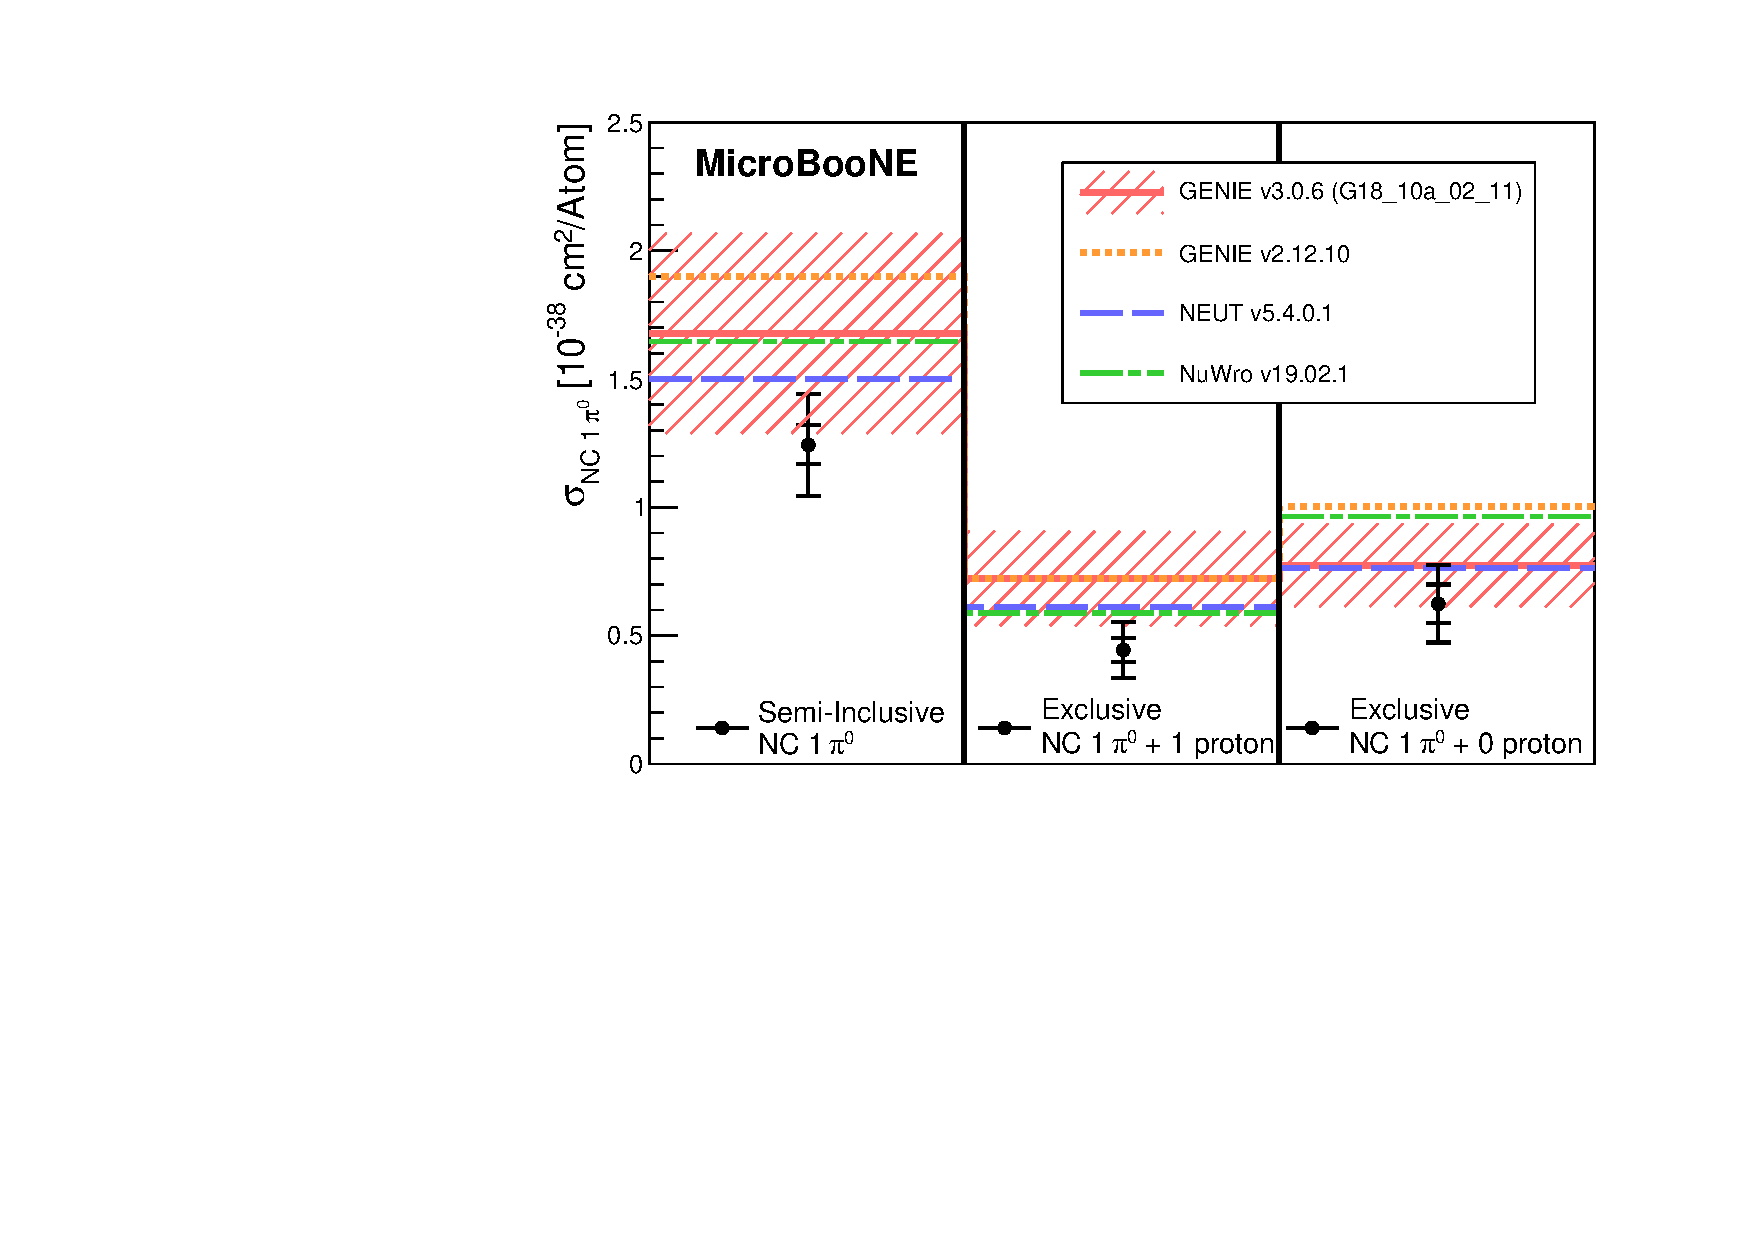
\includegraphics[width=0.49\textwidth]{fig12_NOV_SIMPLE_combined_2g1p_2g0p_simple_XS.pdf}
    \caption{Measured semi-inclusive NC$\pi^0$, exclusive NC$\pi^0$+1p, and exclusive NC$\pi^0$+0p cross sections, each compared to the corresponding \textsc{genie} v3 (G18\_10a\_02\_11) cross section and its uncertainty (shaded red bands) as well as other contemporary neutrino generators. Inner error bars on data points are statistical only; outer are statistical and systematic, summed in quadrature.}
	\label{fig:xsec_comparison}
\end{figure}
%%%%%%%%%%%%%%%%%%%%%%%%%%%%%%%%%%%%%%%%%%%%%%%%%%%%%
%%%%%%%%%%%%%%%%%%%%%%%%%%%%%%%%%%%%%%%%%%%%%%%%%%%%%

%%%%%%%%%%%%%%%%%%%%%%%%%%%%%%%%%%%%%%%%%%%%%%%%%%%%%
%%%%%%%%%%%%% Cross Section Uncertainty Plot
\begin{figure}[h]
	\centering
	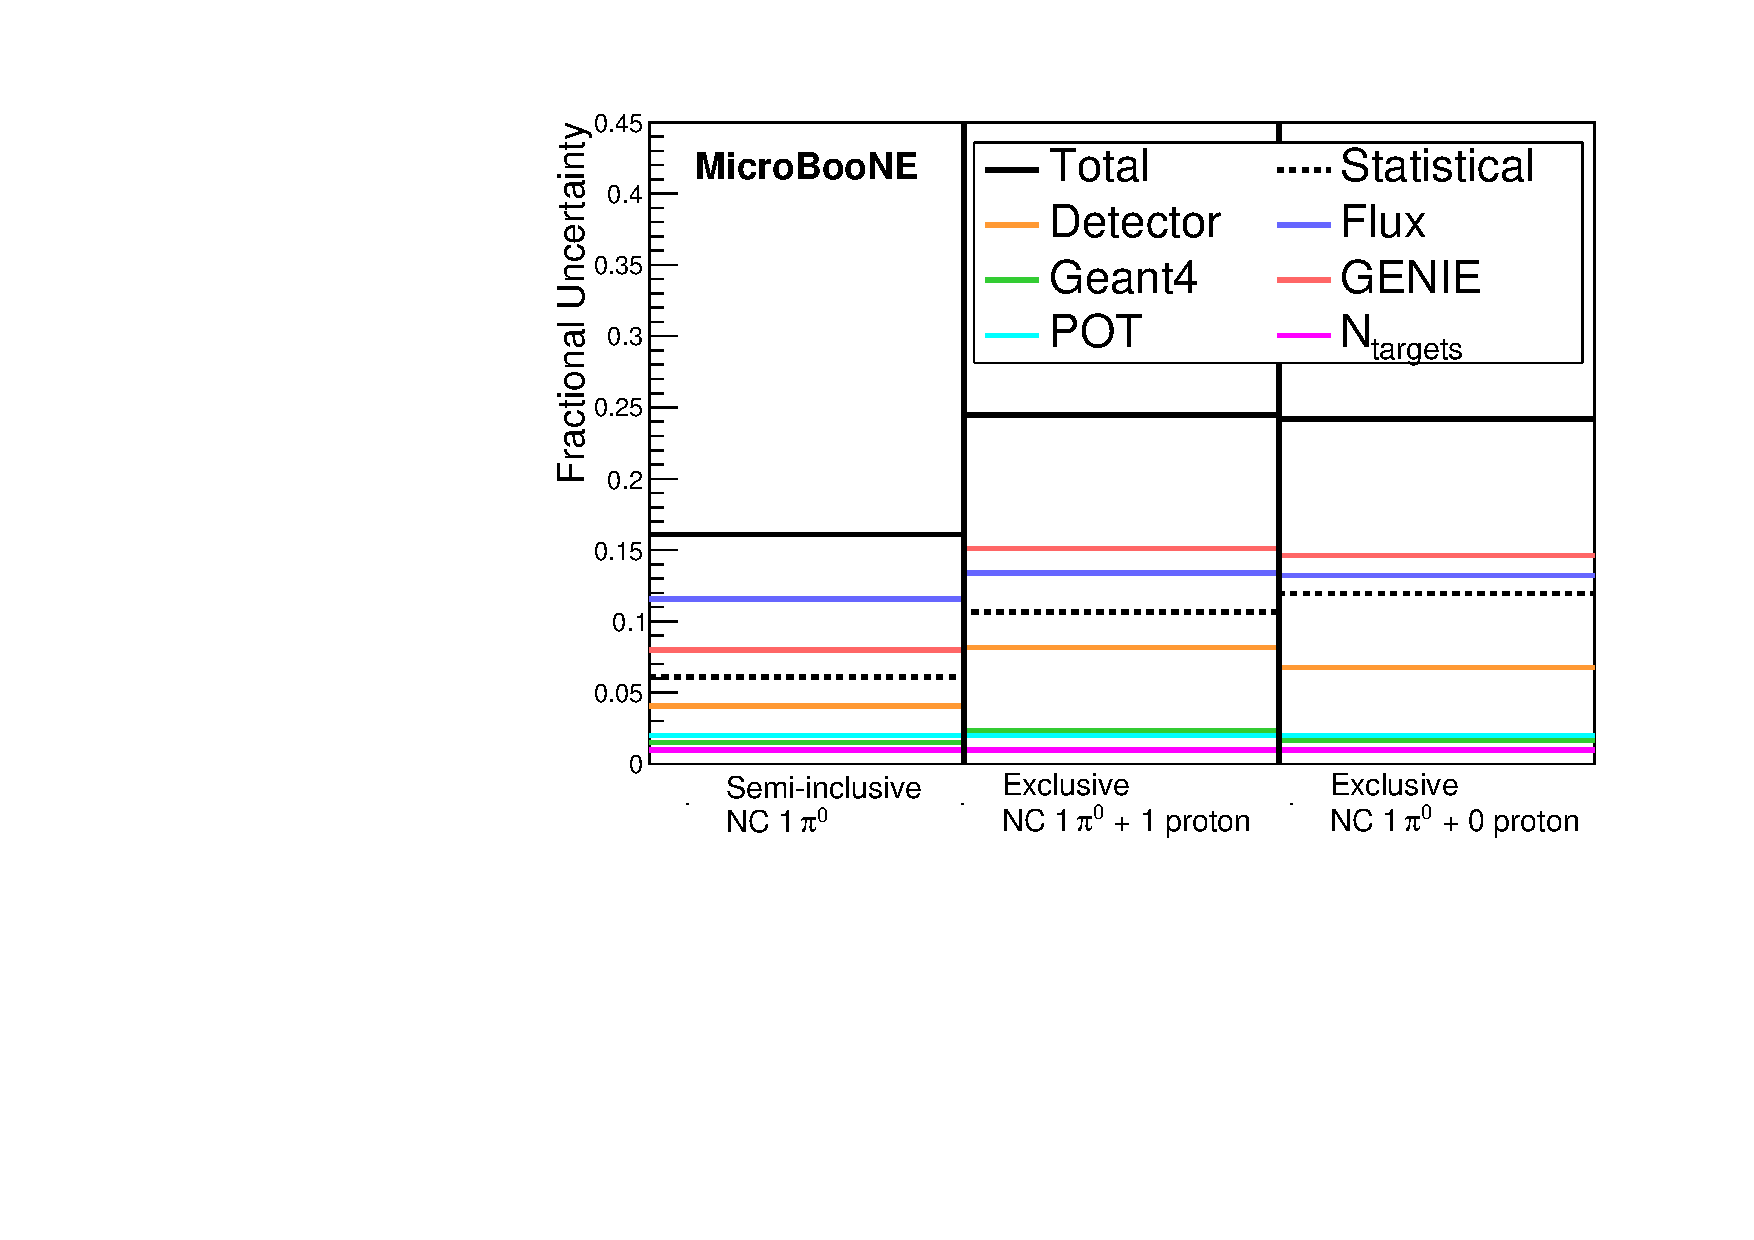
\includegraphics[width=0.49\textwidth]{fig13_errorSummary_xsec_panels.pdf}
     \caption{Error budget for the semi-inclusive NC$\pi^0$, exclusive NC$\pi^0$+1p, and exclusive NC$\pi^0$+0p cross section measurements.}
	\label{fig:xsec_uncertainty}
\end{figure}
%%%%%%%%%%%%%%%%%%%%%%%%%%%%%%%%%%%%%%%%%%%%%%%%%%%%%
%%%%%%%%%%%%%%%%%%%%%%%%%%%%%%%%%%%%%%%%%%%%%%%%%%%%%

To further understand this measurement, it is instructive to compare it to previous experimental measurements of NC$\pi^0$ production. We compare our measurement to that performed by MiniBooNE which operated in the same beamline as MicroBooNE but which utilized a different detector material (mineral oil, CH$_2$) as the neutrino scattering target. In MiniBooNE's  NC $\pi^0$ analysis, they measured NC interactions wherein only one $\pi^0$ and no additional mesons exited the target nucleus (no requirement on the number or identity of outgoing nucleons was made). A final flux-averaged cross section of 4.76 $\pm$ 0.76 $\pm$ 0.05 [$10^{-40}$cm$^2$/nucleon] was reported \cite{MiniBooNE:2009dxl}. We can compare this result to our semi-inclusive result by comparing each to the same neutrino generator. This is shown in Fig.~\ref{fig:compare_uB} where we compare both to the default \textsc{GENIE} v3.0.6 on argon and mineral oil respectively. We observe that while this result on argon lies slightly below the expected central value, both our result and MiniBooNE's agree with \textsc{GENIE} v3.0.6 within assigned uncertainties. 

\begin{figure}[h]
	\centering
	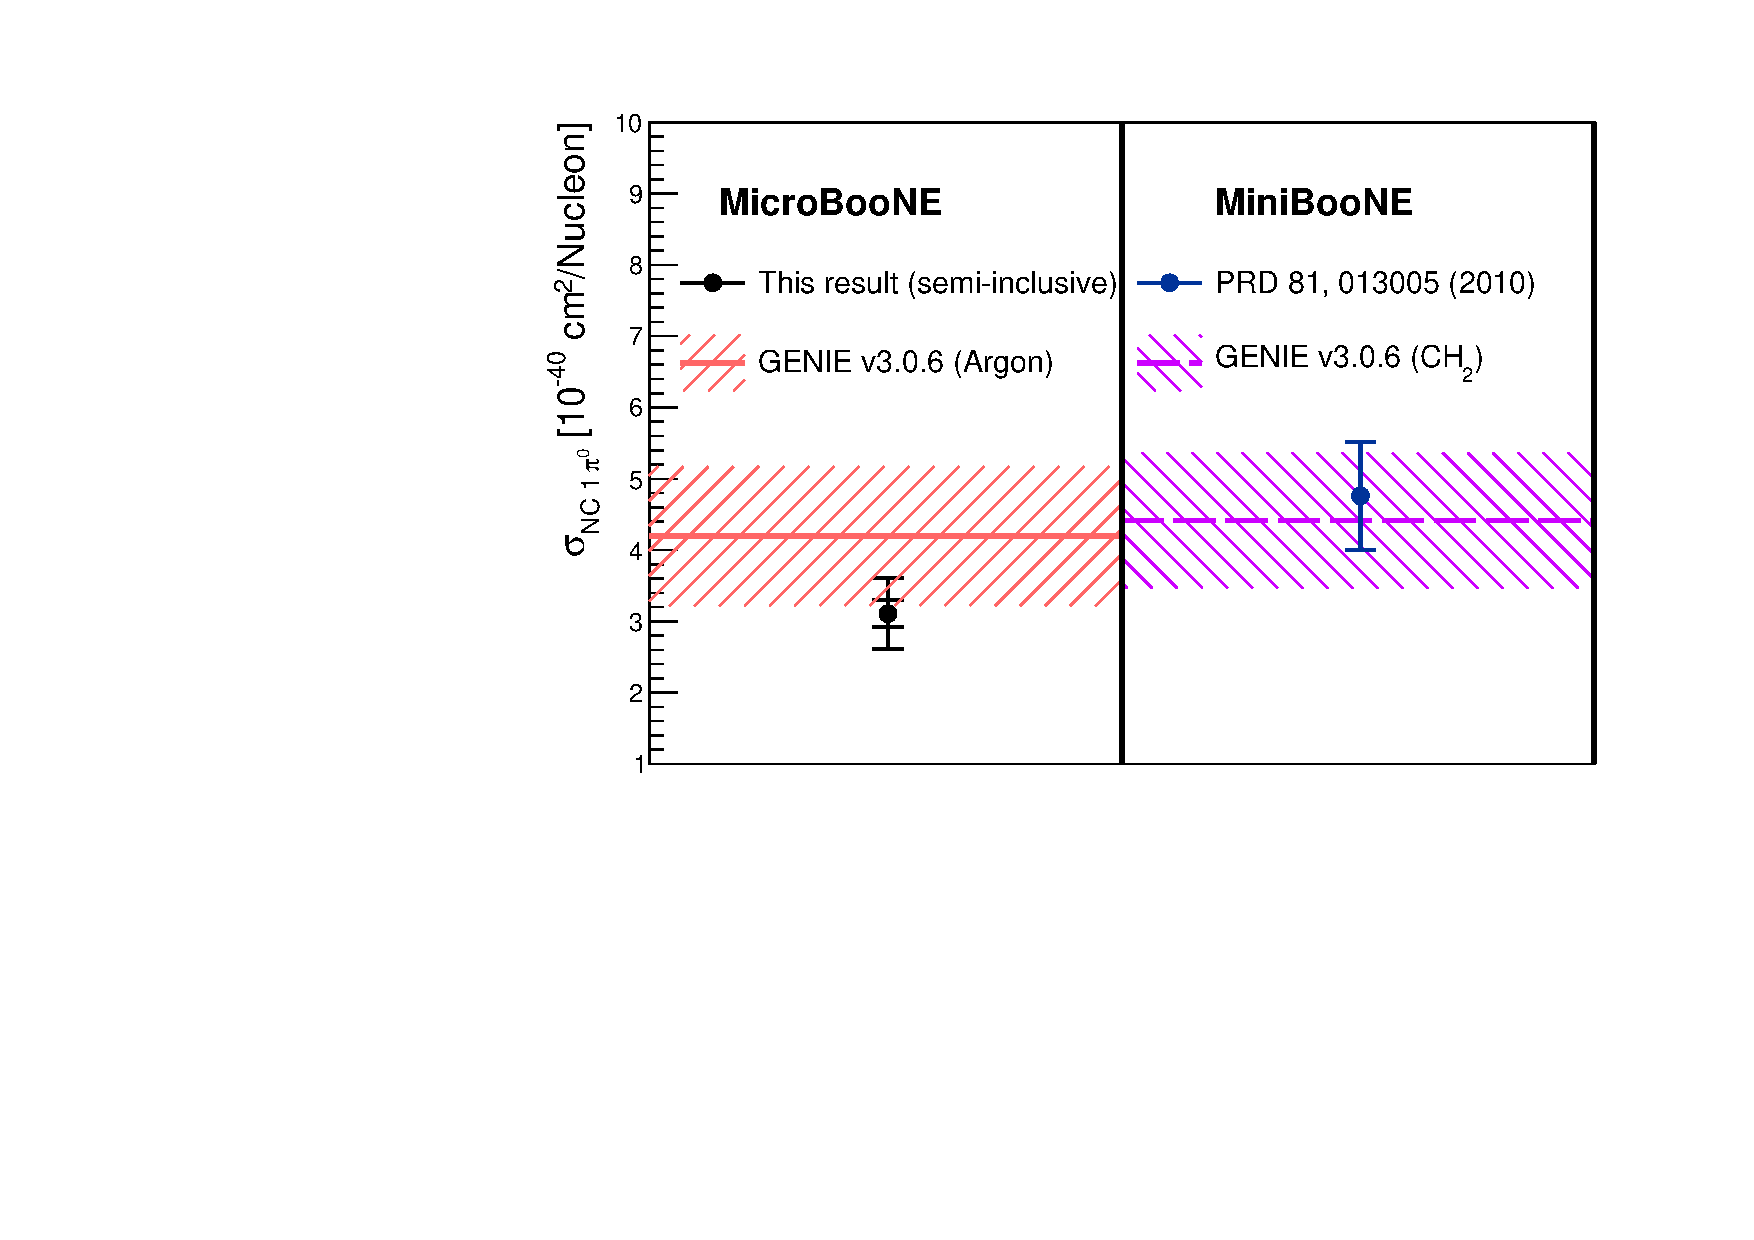
\includegraphics[width=0.49\textwidth]{fig14_compare_uB_v_MB.pdf}
    \caption{Comparison of this semi-inclusive result on argon (left) as well as that from MiniBooNE on mineral oil CH$_2$ (right), to the same \textsc{GENIE} v3.0.6. While the published MiniBooNE result was originally compared to a prediction made using the \textsc{NUANCE} v3 generator \cite{Casper:2002sd}, we have instead generated a prediction using GENIE to aid in a comparison between the two experimental results. MiniBooNE's statistical uncertainty is small and only the systematic error bar is visible. Shaded error bands show \textsc{GENIE} uncertainty only.}
	\label{fig:compare_uB}
\end{figure}